\documentclass[UTF8, a4paper, 11pt]{article}
\usepackage{subfigure}
\usepackage[UTF8, scheme=plain]{ctex}
\usepackage{fontspec}
\usepackage{float}
\usepackage{amsmath}
\newtheorem{myDef}{Definition}
\usepackage{graphicx}
\usepackage{geometry}
\usepackage{listings}
\usepackage{xcolor}
\usepackage{caption}
\geometry{scale=0.8}
\linespread{1.5}
\usepackage{hyperref}
\usepackage{color}
\usepackage{fontspec}
\usepackage{enumitem}
\usepackage[linesnumbered,boxed]{algorithm2e}    
\usepackage{xeCJK}
\usepackage{indentfirst} 
\graphicspath{{Pics/}} 	% 在于.tex同级的目录下创建名为pic的文件夹,存放图片


\setlength{\parindent}{2em}

\lstset{
    language={C},
    frame=shadowbox,
    breaklines=true,
    numbers=left,
    backgroundcolor=\color[RGB]{245,245,244},
    rulesepcolor=\color{red!20!green!20!blue!20},
    numberstyle={\color[RGB]{0,192,192}\tiny},
    basicstyle=\footnotesize \fontspec{Source Code Pro}
}
\setenumerate[1]{itemsep=0pt,partopsep=0pt,parsep=\parskip,topsep=0pt}
\setitemize[1]{itemsep=0pt,partopsep=0pt,parsep=\parskip,topsep=0pt}
\setdescription{itemsep=0pt,partopsep=0pt,parsep=\parskip,topsep=0pt}


\title{	
\normalfont \normalsize
\textsc{School of Data and Computer Science, Sun Yat-sen University} \\ [25pt] %textsc small capital letters
\rule{\textwidth}{0.5pt} \\[0.4cm] % Thin top horizontal rule
\huge 数电实验1\\ % The assignment title
\rule{\textwidth}{2pt} \\[0.5cm] % Thick bottom horizontal rule
\author{18308045 谷正阳}
\date{\normalsize\today}
}

\begin{document}
\maketitle
\tableofcontents
\newpage
\section{仿真实验}
\subsection{电路图}
\begin{figure}[H]
    \centering
    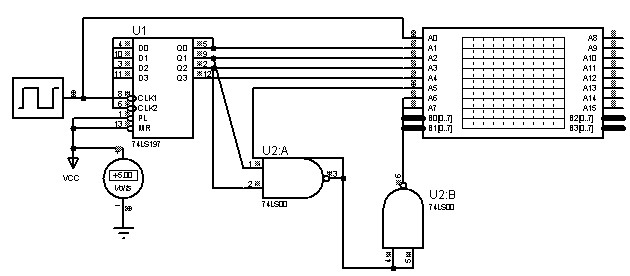
\includegraphics[width=0.8\textwidth]{电路图.jpg}
\end{figure}
老师课上提示,将与非门两个输入端串联成一个输入端,就是非门。而将非门串联到与非门的输出端就是与门。

电路图中,A0是10kHz时钟脉冲,A1、A2、A3、A4分别是Q0、Q1、Q2、Q3,A2、A3是与非门/与门的输入,A5是与非门的输出,A6是与门的输出。
\subsection{仿真结果}
\begin{figure}[H]
    \centering
    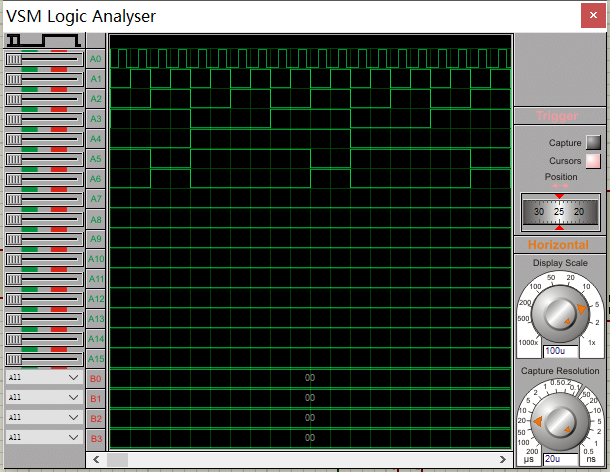
\includegraphics[width=0.8\textwidth]{analyser.png}
\end{figure}
可以看出,A1、A2、A3、A4构成16进制计数器,A2、A3、A4构成8进制计数器,$\overline{A2\cdot A3}=A5$,$A2\cdot A3=A6$。
\section{实验箱实验}
\subsection{与非门静态实验}
\begin{figure}[H] %这里使用的是强制位置,除非真的放不下,不然就是写在哪里图就放在哪里,不会乱动
	\centering  %图片全局居中
	\vspace{-0.35cm} %设置与上面正文的距离
	\subfigtopskip=2pt %设置子图与上面正文或别的内容的距离
	\subfigbottomskip=2pt %设置第二行子图与第一行子图的距离,即下面的头与上面的脚的距离
	\subfigcapskip=2pt %设置子图与子标题之间的距离
	\subfigure[$\overline{0\cdot0}=1$]{
		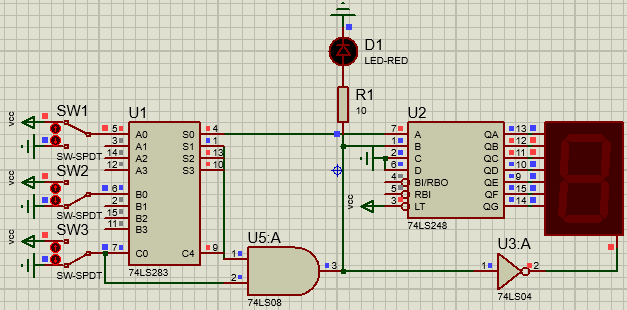
\includegraphics[width=0.5\linewidth,angle=-90]{001.jpg}}
	\quad %默认情况下两个子图之间空的较少,使用这个命令加大宽度
	\subfigure[$\overline{0\cdot1}=1$]{
		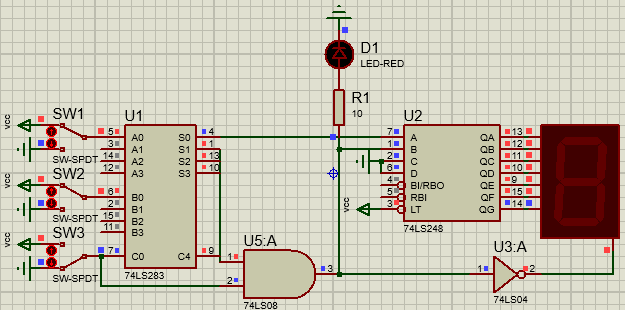
\includegraphics[width=0.5\linewidth,angle=-90]{011.jpg}}
	\\%这里是空了一行,能够实现强制将四张图分成两行两列显示,而不是放不下图了再换行,使用\\也行。
	\subfigure[$\overline{1\cdot0}=1$]{
		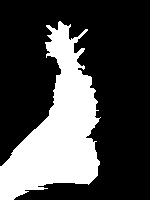
\includegraphics[width=0.5\linewidth,angle=-90]{101.jpg}}
	\quad
	\subfigure[$\overline{1\cdot1}=0$]{
		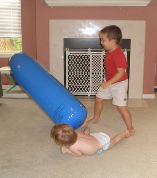
\includegraphics[width=0.5\linewidth,angle=-90]{110.jpg}}
\end{figure}
\subsection{与门静态实验}
\begin{figure}[H] %这里使用的是强制位置,除非真的放不下,不然就是写在哪里图就放在哪里,不会乱动
	\centering  %图片全局居中
	\vspace{-0.35cm} %设置与上面正文的距离
	\subfigtopskip=2pt %设置子图与上面正文或别的内容的距离
	\subfigbottomskip=2pt %设置第二行子图与第一行子图的距离,即下面的头与上面的脚的距离
	\subfigcapskip=2pt %设置子图与子标题之间的距离
	\subfigure[$0\cdot0=0$]{
		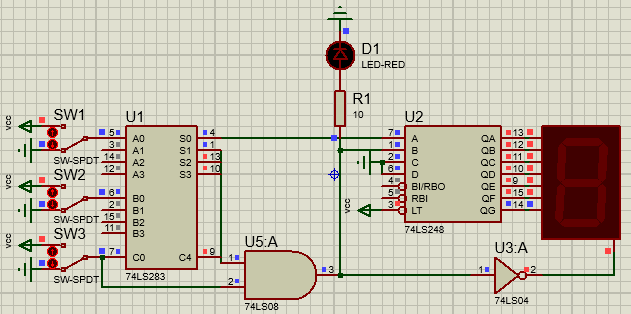
\includegraphics[width=0.5\linewidth,angle=-90]{000.jpg}}
	\quad %默认情况下两个子图之间空的较少,使用这个命令加大宽度
	\subfigure[$0\cdot1=0$]{
		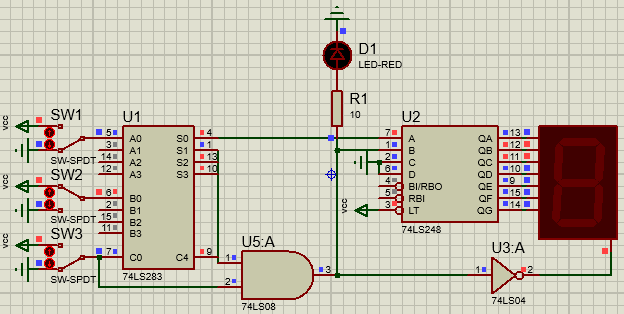
\includegraphics[width=0.5\linewidth,angle=-90]{010.jpg}}
	\\%这里是空了一行,能够实现强制将四张图分成两行两列显示,而不是放不下图了再换行,使用\\也行。
	\subfigure[$1\cdot0=0$]{
		
\includegraphics[width=0.5\linewidth,angle=-90]{100.jpg}}
	\quad
	\subfigure[$1\cdot1=1$]{
		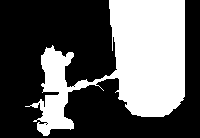
\includegraphics[width=0.5\linewidth,angle=-90]{111.jpg}}
\end{figure}
\subsection{与非门动态实验}
在此只保留了用到的信号,CLK1,Q1,Q2和输出。
\begin{figure}[H]
    \centering
    \includegraphics[width=0.8\textwidth]{与非.jpg}
\end{figure}
\subsection{与门动态实验}
在此只保留了用到的信号,CLK1,Q1,Q2和输出。
\begin{figure}[H]
    \centering
    \includegraphics[width=0.8\textwidth]{与.jpg}
\end{figure}
\section{实验总结}
本次实验学习了Proteus和实验箱的使用方法,并学习了8/16进制计数器74LS197的使用方法,并学会了运用74LS00搭建与非门、非门和与门的方法。
%\clearpage
%\bibliography{E:/Papers/LiuLab}
%\bibliographystyle{apalike}
\end{document}
%%% Local Variables:
%%% mode: latex
%%% TeX-master: t
%%% End:
